%-----------------------------------LICENSE------------------------------------%
%   This file is part of Mathematics-and-Physics.                              %
%                                                                              %
%   Mathematics-and-Physics is free software: you can redistribute it and/or   %
%   modify it it under the terms of the GNU General Public License as          %
%   published by the Free Software Foundation, either version 3 of the         %
%   License, or (at your option) any later version.                            %
%                                                                              %
%   Mathematics-and-Physics is distributed in the hope that it will be useful, %
%   but WITHOUT ANY WARRANTY; without even the implied warranty of             %
%   MERCHANTABILITY or FITNESS FOR A PARTICULAR PURPOSE.  See the              %
%   GNU General Public License for more details.                               %
%                                                                              %
%   You should have received a copy of the GNU General Public License along    %
%   with Mathematics-and-Physics.  If not, see <https://www.gnu.org/licenses/>.%
%------------------------------------------------------------------------------%

%   Use the standalone class for displaying the tikz image on a small PDF.
\documentclass[crop, tikz]{standalone}

%   Import the tikz package to use for the drawing.
\usepackage{tikz}

%   The arrows package is used for the LaTeX arrow.
\usetikzlibrary{arrows.meta}

%   Begin the document.
\begin{document}

    %   Begin the drawing.
    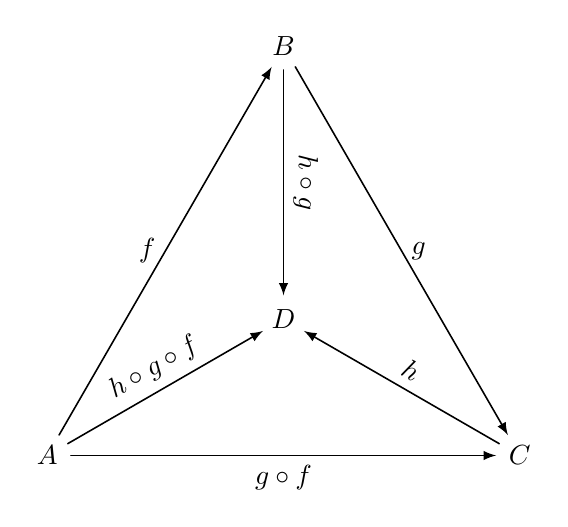
\begin{tikzpicture}[%
        >=latex,%
        line cap=round,%
        line width=0.2mm%
    ]
        %   Mark the four points on the diagram.
        \coordinate (A) at (-3.0, 0.000);
        \coordinate (B) at ( 0.0, 5.196);
        \coordinate (C) at ( 3.0, 0.000);
        \coordinate (D) at ( 0.0, 1.732);

        %   Label the points.
        \node at (A) {$A$};
        \node at (B) {$B$};
        \node at (C) {$C$};
        \node at (D) {$D$};

        %   Draw arrows between the nodes.
        \begin{scope}[->, shorten <=3mm, shorten >=3mm] 
            \draw (A) to node[left] {$f$} (B);
            \draw (B) to node[right] {$g$} (C);
            \draw (A) to node[below] {$g\circ{f}$} (C);
            \draw (C) to node[above, rotate=-30] {$h$} (D);
            \draw (B) to node[above, rotate=-90] {$h\circ{g}$} (D);
            \draw (A) to node[above, rotate=30] {$h\circ{g}\circ{f}$} (D);
        \end{scope}
    \end{tikzpicture}
\end{document}
